\chapter{deeplearning}
\section{降维}
\subsection{自编码}
人工神经网络(ANN)本身就是具有层次结构的系统,如果给定一个神经网络,我们假设其输出与输入是相同的,然后训练调整其参数,得到每一层中的权重。自然地,我们就得到了输入I的几种不同表示(每一层代表一种表示),这些表示就是特征。在研究中可以发现,如果在原有的特征中加入这些自动学习得到的特征可以大大提高精确度,甚至在分类问题中比目前最好的分类算法效果还要好!这种方法称为AutoEncoder(自动编码器)。自动编码器就是一种尽可能复现输入信号的神经网络。为了实现这种复现,自动编码器就必须捕捉可以代表输入数据的最重要的因素,就像PCA那样,找到可以代表原信息的主要成分。
我们将input输入一个encoder编码器,就会得到一个code,这个code也就是输入的一个表示,那么我们怎么知道这个code表示的就是input呢?我们加一个decoder解码器,这时候decoder就会输出一个信息,那么如果输出的这个信息和一开始的输入信号input是很像的(理想情况下就是一样的),那很明显,我们就有理由相信这个code是靠谱的。所以,我们就通过调整encoder和decoder的参数,使得重构误差最小,这时候我们就得到了输入input信号的第一个表示了,也就是编码code了。因为是无标签数据,所以误差的来源就是直接重构后与原输入相比得到。
\subsection{自动降噪编码}
以一定的概率分布擦出原始数据(将数据置为0),这样操作后的数据称为破损数据,这样的数据有两个作用:
\begin{enumerate}
\item 通过破损数据和非破损数据相比,破损数据训练出来的权重噪声小(可能不小心删除了噪声)。
\item 破损数据一定程度上减轻了训练数据和测试数据之间的代沟。由于数据部分被擦除,因而训练出来的权重的健壮性就提高了。
\end{enumerate}
\subsection{手写体数据自编码}
\begin{tikzpicture}
  \SetGraphUnit{5}
  \Vertex{B}
  \WE(B){Origin Data}
  \EA(B){Processed Data}
  \Edge[label = encode1,color = blue](Origin Data)(B)
  \Edge[label = encode2,color = blue](B)(Processed Data)
  \Edge[label = decode2,color = red](Processed Data)(B)
  \Edge[label = decode1,color = red](B)(Origin Data)
  \tikzset{EdgeStyle/.append style = {bend left = 50}}
  \Edge[label = encode,color=blue](Origin Data)(Processed Data)
  \Edge[label = decode,color=red](Processed Data)(Origin Data)
\end{tikzpicture}

\begin{python}
import tensorflow as tf
import matplotlib.pyplot as plt
data_path = '/home/hpc/文档/mnist_tutorial/mnist'

from tensorflow.examples.tutorials.mnist import input_data
mnist = input_data.read_data_sets(data_path, one_hot=False)


# Visualize decoder setting
learning_rate = 0.01
training_epochs = 5
batch_size = 256
display_step = 1
examples_to_show = 10

n_input = 784  # MNIST data input (img shape: 28*28)

x = tf.placeholder(tf.float32,[None,n_input])

n_hidden_1 = 256
n_hidden_2 = 128
weights = {
    'encode_h1':tf.Variable(tf.random_normal([n_input,n_hidden_1])),
    'encode_h2':tf.Variable(tf.random_normal([n_hidden_1,n_hidden_2])),
    'decode_h2':tf.Variable(tf.random_normal([n_hidden_2,n_hidden_1])),
    'decode_h1':tf.Variable(tf.random_normal([n_hidden_1,n_input]))
}
bias = {'encode_h1':tf.Variable(tf.random_normal([n_hidden_1])),
    'encode_h2':tf.Variable(tf.random_normal([n_hidden_2])),
    'decode_h2':tf.Variable(tf.random_normal([n_hidden_1])),
    'decode_h1':tf.Variable(tf.random_normal([n_input]))

}
def encode(x):
    layer_1 = tf.nn.sigmoid(tf.add(tf.matmul(x,weights['encode_h1']),bias['encode_h1']))
    layer_2 = tf.nn.sigmoid(tf.add(tf.matmul(layer_1,weights['encode_h2']),bias['encode_h2']))
    return layer_2

def decode(x):
    layer_1 = tf.nn.sigmoid(tf.add(tf.matmul(x,weights['decode_h2']),bias['decode_h2']))
    layer_2 = tf.nn.sigmoid(tf.add(tf.matmul(layer_1,weights['decode_h1']),bias['decode_h1']))
    return layer_2



encode_op = encode(x)
decode_op = decode(encode_op)
y_pred = decode_op
y_true = x
cost = tf.reduce_mean(tf.square(y_pred-y_true))
optimizer = tf.train.AdamOptimizer(learning_rate).minimize(cost)

with tf.Session() as sess:
    init = tf.global_variables_initializer()
    sess.run(init)
    total_batch = int(mnist.train.num_examples/batch_size)
    for epoch in range(training_epochs):
        for i in range(total_batch):
            batch_xs,batch_ys = mnist.train.next_batch(batch_size)
            _, c = sess.run([optimizer, cost], feed_dict={x: batch_xs})
        if epoch%display_step==0:
            print("Epoch:",'%04d'%(epoch+1),'cost=','{:.9f}'.format(c))
    print('Optimize finish')
    encode_decode = sess.run(y_pred,feed_dict={x:mnist.test.images[:examples_to_show]})
    f,a = plt.subplots(2,10,figsize=(10,2))
    for i in range(examples_to_show):
        a[0][i].imshow(sess.run(tf.reshape(mnist.test.images[i],[28,28])))
        a[1][i].imshow(sess.run(tf.reshape(encode_decode[i],[28,28])))
    plt.savefig('auto_encode.png',dpi=800)
\end{python}
\begin{center}
\begin{figure}[H]
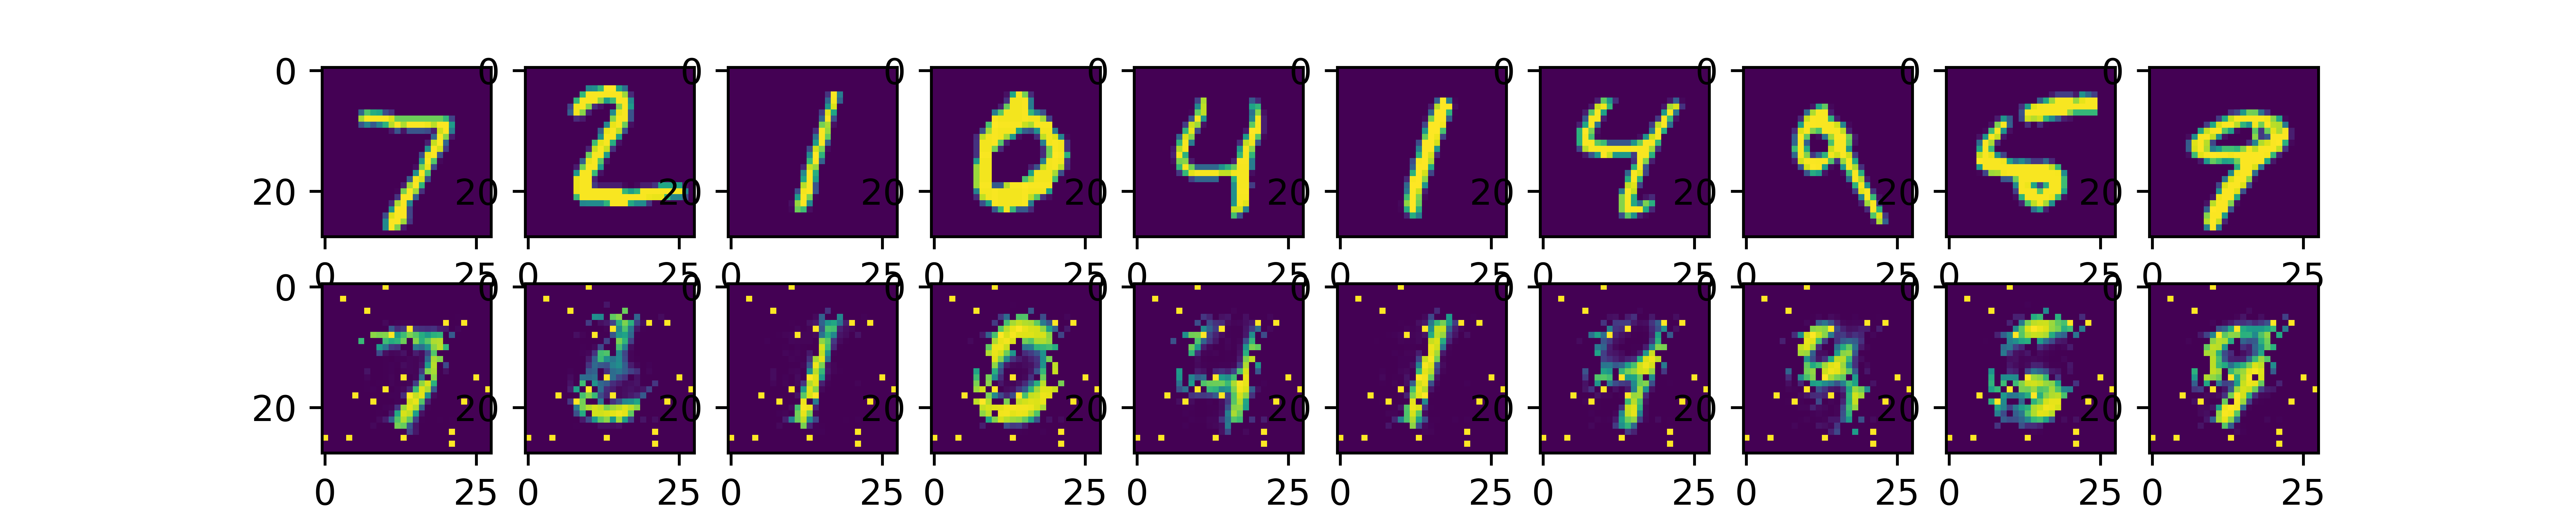
\includegraphics[scale=0.5]{auto_encode.png}
\caption{原图和自编码解码后的图像}
\end{figure}
\end{center}
编码器输出可视化:
\begin{python}
import tensorflow as tf
import matplotlib.pyplot as plt

from tensorflow.examples.tutorials.mnist import input_data
path = '/home/hpc/文档/mnist_tutorial/mnist'
mnist = input_data.read_data_sets(path, one_hot=False)

learning_rate = 0.01
training_epochs = 5
batch_size = 256
display_step = 1
examples_to_show = 10

n_input = 784  # MNIST data input (img shape: 28*28)

X = tf.placeholder("float", [None, n_input])

n_hidden_1 = 256 # 1st layer num features
n_hidden_2 = 128 # 2nd layer num features

learning_rate = 0.01    # 0.01 this learning rate will be better! Tested
training_epochs = 10
batch_size = 256
display_step = 1
n_input = 784  # MNIST data input (img shape: 28*28)
X = tf.placeholder("float", [None, n_input])
n_hidden_1 = 128
n_hidden_2 = 64
n_hidden_3 = 10
n_hidden_4 = 2
weights = {
    'encoder_h1': tf.Variable(tf.truncated_normal([n_input, n_hidden_1],)),
    'encoder_h2': tf.Variable(tf.truncated_normal([n_hidden_1, n_hidden_2],)),
    'encoder_h3': tf.Variable(tf.truncated_normal([n_hidden_2, n_hidden_3],)),
    'encoder_h4': tf.Variable(tf.truncated_normal([n_hidden_3, n_hidden_4],)),
    'decoder_h1': tf.Variable(tf.truncated_normal([n_hidden_4, n_hidden_3],)),
    'decoder_h2': tf.Variable(tf.truncated_normal([n_hidden_3, n_hidden_2],)),
    'decoder_h3': tf.Variable(tf.truncated_normal([n_hidden_2, n_hidden_1],)),
    'decoder_h4': tf.Variable(tf.truncated_normal([n_hidden_1, n_input],)),
}
biases = {
    'encoder_b1': tf.Variable(tf.random_normal([n_hidden_1])),
    'encoder_b2': tf.Variable(tf.random_normal([n_hidden_2])),
    'encoder_b3': tf.Variable(tf.random_normal([n_hidden_3])),
    'encoder_b4': tf.Variable(tf.random_normal([n_hidden_4])),
    'decoder_b1': tf.Variable(tf.random_normal([n_hidden_3])),
    'decoder_b2': tf.Variable(tf.random_normal([n_hidden_2])),
    'decoder_b3': tf.Variable(tf.random_normal([n_hidden_1])),
    'decoder_b4': tf.Variable(tf.random_normal([n_input])),
}
def encoder(x):
    layer_1 = tf.nn.sigmoid(tf.add(tf.matmul(x, weights['encoder_h1']),
                                   biases['encoder_b1']))
    layer_2 = tf.nn.sigmoid(tf.add(tf.matmul(layer_1, weights['encoder_h2']),
                                   biases['encoder_b2']))
    layer_3 = tf.nn.sigmoid(tf.add(tf.matmul(layer_2, weights['encoder_h3']),
                                   biases['encoder_b3']))
    layer_4 = tf.add(tf.matmul(layer_3, weights['encoder_h4']),
                                    biases['encoder_b4'])
    return layer_4
def decoder(x):
    layer_1 = tf.nn.sigmoid(tf.add(tf.matmul(x, weights['decoder_h1']),
                                   biases['decoder_b1']))
    layer_2 = tf.nn.sigmoid(tf.add(tf.matmul(layer_1, weights['decoder_h2']),
                                   biases['decoder_b2']))
    layer_3 = tf.nn.sigmoid(tf.add(tf.matmul(layer_2, weights['decoder_h3']),
                                biases['decoder_b3']))
    layer_4 = tf.nn.sigmoid(tf.add(tf.matmul(layer_3, weights['decoder_h4']),
                                biases['decoder_b4']))
    return layer_4

encoder_op = encoder(X)
decoder_op = decoder(encoder_op)

y_pred = decoder_op
y_true = X

cost = tf.reduce_mean(tf.pow(y_true - y_pred, 2))
optimizer = tf.train.AdamOptimizer(learning_rate).minimize(cost)


with tf.Session() as sess:
    init = tf.global_variables_initializer()
    sess.run(init)
    total_batch = int(mnist.train.num_examples/batch_size)
    for epoch in range(training_epochs):
        for i in range(total_batch):
            batch_xs, batch_ys = mnist.train.next_batch(batch_size)  # max(x) = 1, min(x) = 0
            _, c = sess.run([optimizer, cost], feed_dict={X: batch_xs})
        if epoch % display_step == 0:
            print("Epoch:", '%04d' % (epoch+1),
                  "cost=", "{:.9f}".format(c))
    print("Optimization Finished!")
    encode_decode = sess.run(
        y_pred, feed_dict={X: mnist.test.images[:examples_to_show]})
    encoder_result = sess.run(encoder_op, feed_dict={X: mnist.test.images})
    plt.scatter(encoder_result[:, 0], encoder_result[:, 1], c=mnist.test.labels)
    plt.title('encode output')
    plt.colorbar()
    plt.savefig('auto_encode_v.png',dpi=800)
\end{python}

\begin{center}
\begin{figure}[H]
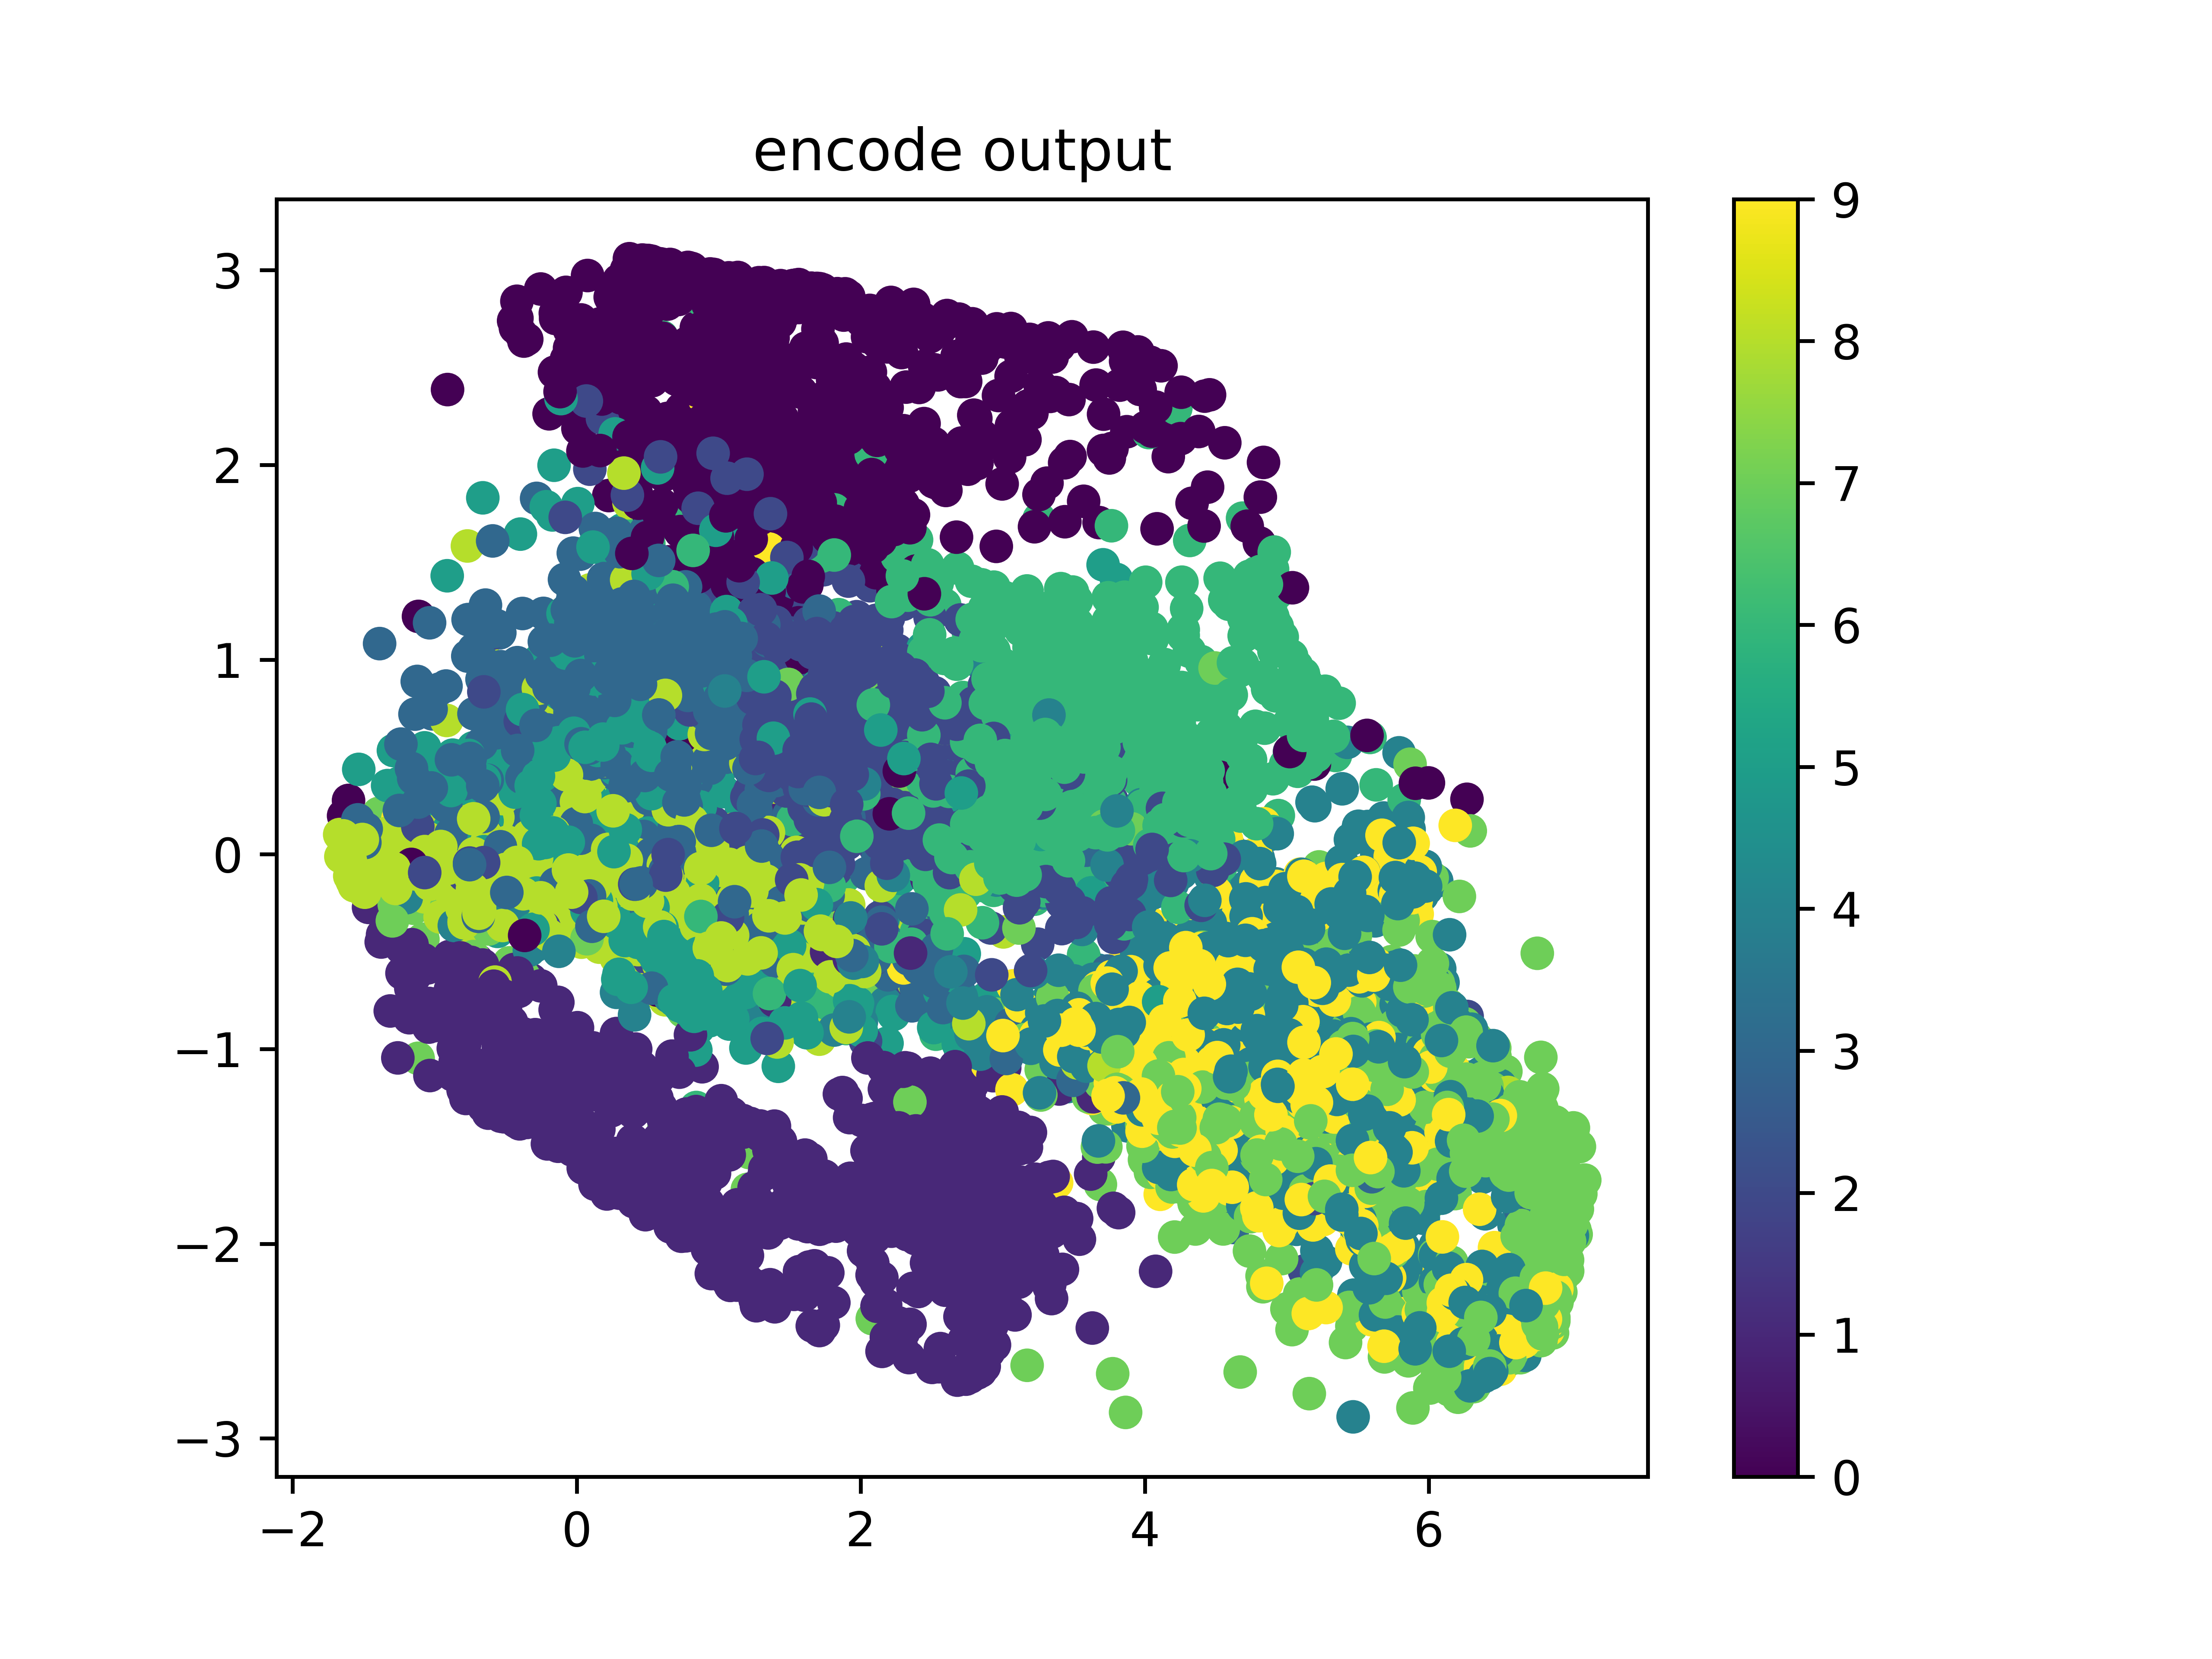
\includegraphics[scale=0.7]{auto_encode_v.png}
\end{figure}
\end{center}
\section{稀疏编码}
稀疏编码算法是一种无监督学习方法,它用来寻找一组“超完备”基向量来更高效地表示样本数据。稀疏编码算法的目的就是找到一组基向量 $\mathbf{\phi}_i$ ,使得我们能将输入向量 $\mathbf{x}$ 表示为这些基向量的线性组合:
\begin{align}
\mathbf{x} = \sum_{i=1}^k a_i \mathbf{\phi}_{i} 
\end{align}
虽然形如主成分分析技术(PCA)能使我们方便地找到一组“完备”基向量,但是这里我们想要做的是找到一组“超完备”基向量来表示输入向量 $\mathbf{x}\in\mathbb{R}^n$ (也就是说,k > n)。超完备基的好处是它们能更有效地找出隐含在输入数据内部的结构与模式。然而,对于超完备基来说,系数$a_i$不再由输入向量 $\mathbf{x}$ 唯一确定。因此,在稀疏编码算法中,我们另加了一个评判标准“稀疏性”来解决因超完备而导致的退化(degeneracy)问题。

这里,我们把“稀疏性”定义为:只有很少的几个非零元素或只有很少的几个远大于零的元素。要求系数$a_i$ 是稀疏的意思就是说:对于一组输入向量,我们只想有尽可能少的几个系数远大于零。选择使用具有稀疏性的分量来表示我们的输入数据是有原因的,因为绝大多数的感官数据,比如自然图像,可以被表示成少量基本元素的叠加,在图像中这些基本元素可以是面或者线。同时,比如与初级视觉皮层的类比过程也因此得到了提升。

我们把有 m 个输入向量的稀疏编码代价函数定义为:
\begin{align}
\text{minimize}_{a^{(j)}_i,\mathbf{\phi}_{i}} \sum_{j=1}^{m} \left|\left| \mathbf{x}^{(j)} - \sum_{i=1}^k a^{(j)}_i \mathbf{\phi}_{i}\right|\right|^{2} + \lambda \sum_{i=1}^{k}S(a^{(j)}_i)
\end{align}

此处 S(.) 是一个稀疏代价函数,由它来对远大于零的 $a_i$ 进行“惩罚”。我们可以把稀疏编码目标函式的第一项解释为一个重构项,这一项迫使稀疏编码算法能为输入向量 $\mathbf{x}$ 提供一个高拟合度的线性表达式,而公式第二项即“稀疏惩罚”项,它使 $\mathbf{x}$ 的表达式变得“稀疏”。常量$\lambda$是一个变换量,由它来控制这两项式子的相对重要性。

虽然“稀疏性”的最直接测度标准是 "L0" 范式$(S(a_i) = \mathbf{1}(|a_i|>0))$,但这是不可微分的,而且通常很难进行优化。在实际中,稀疏代价函数 S(.) 的普遍选择是L1 范式代价函数 $S(a_i)=\left|a_i\right|_1$  及对数代价函数 $S(a_i)=\log(1+a_i^2)$ 。

此外,很有可能因为减小 $a_i$ 或增加 $\mathbf{\phi}_i$ 至很大的常量,使得稀疏惩罚变得非常小。为防止此类事件发生,我们将限制 $\left|\left|\mathbf{\phi}\right|\right|^2$ 要小于某常量 C 。包含了限制条件的稀疏编码代价函数的完整形式如下:
\begin{equation}
\text{minimize}_{a_i^{(j)},\phi_i}\Sigma_{j=1}^m\|x^{(j)}-\Sigma_{i=1}^ka_i^{(j)}\phi_i\|^2+\lambda\Sigma_{i=1}^kS(s_i^{(j)})\quad\|\phi_i\|^2\leq C,\forall i=1,\ldots,k
\end{equation}
\subsection{稀疏编码的概率表示}
到目前为止,我们所考虑的稀疏编码,是为了寻找到一个稀疏的、超完备基向量集,来覆盖我们的输入数据空间。现在换一种方式,我们可以从概率的角度出发,将稀疏编码算法当作一种“生成模型”。

我们将自然图像建模问题看成是一种线性叠加,叠加元素包括 k 个独立的源特征 $\mathbf{\phi}_i$ 以及加性噪声 ν :
\begin{align}
\mathbf{x} = \sum_{i=1}^k a_i \mathbf{\phi}_{i} + \nu(\mathbf{x})
\end{align}

我们的目标是找到一组特征基向量 $\mathbf{\phi}$ ,它使得图像的分布函数 $P(\mathbf{x}\mid\mathbf{\phi})$ 尽可能地近似于输入数据的经验分布函数 $P^*(\mathbf{x})$ 。一种实现方式是,最小化 $P^*(\mathbf{x})$ 与 $P(\mathbf{x}\mid\mathbf{\phi})$ 之间的 KL 散度,此 KL 散度表示如下:
\begin{align}
D(P^*(\mathbf{x})||P(\mathbf{x}\mid\mathbf{\phi})) = \int P^*(\mathbf{x}) \log \left(\frac{P^*(\mathbf{x})}{P(\mathbf{x}\mid\mathbf{\phi})}\right)d\mathbf{x}
\end{align}

因为无论我们如何选择 $\mathbf{\phi}$ ,经验分布函数 $P^*(\mathbf{x})$ 都是常量,也就是说我们只需要最大化对数似然函数 $P(\mathbf{x}\mid\mathbf{\phi})$ 。 假设v是具有方差$\sigma^2$的高斯白噪声,则有下式:
\begin{align}
P(\mathbf{x} \mid \mathbf{a}, \mathbf{\phi}) = \frac{1}{Z} \exp\left(- \frac{(\mathbf{x}-\sum^{k}_{i=1} a_i \mathbf{\phi}_{i})^2}{2\sigma^2}\right)
\end{align}

为了确定分布 $P(\mathbf{x}\mid\mathbf{\phi})$ ,我们需要指定先验分布 $P(\mathbf{a})$ 。假定我们的特征变量是独立的,我们就可以将先验概率分解为:
\begin{align}
P(\mathbf{a}) = \prod_{i=1}^{k} P(a_i)
\end{align}

此时,我们将“稀疏”假设加入进来——假设任何一幅图像都是由相对较少的一些源特征组合起来的。因此,我们希望$a_i$的概率分布在零值附近是凸起的,而且峰值很高。一个方便的参数化先验分布就是:
\begin{align}
P(a_i) = \frac{1}{Z}\exp(-\beta S(a_i))
\end{align}

这里$S(a_i)$是决定先验分布的形状的函数。

当定义了 $P(\mathbf{x} \mid \mathbf{a} , \mathbf{\phi})$ 和  $P(\mathbf{a})$ 后,我们就可以写出在由 $\mathbf{\phi}$ 定义的模型之下的数据 $\mathbf{x}$ 的概率分布:
\begin{align}
P(\mathbf{x} \mid \mathbf{\phi}) = \int P(\mathbf{x} \mid \mathbf{a}, \mathbf{\phi}) P(\mathbf{a}) d\mathbf{a}
\end{align}

那么,我们的问题就简化为寻找:
\begin{align}
\mathbf{\phi}^*=\text{argmax}_{\mathbf{\phi}} < \log(P(\mathbf{x} \mid \mathbf{\phi})) >
\end{align}

这里 < . > 表示的是输入数据的期望值。

不幸的是,通过对 $\mathbf{a}$ 的积分计算 $P(\mathbf{x} \mid \mathbf{\phi})$ 通常是难以实现的。虽然如此,我们注意到如果$ P(\mathbf{x} \mid \mathbf{\phi}) $的分布(对于相应的 $\mathbf{a}$ )足够陡峭的话,我们就可以用$ P(\mathbf{x} \mid \mathbf{\phi})$ 的最大值来估算以上积分。估算方法如下:
\begin{align}
\mathbf{\phi}^{*'}=\text{argmax}_{\mathbf{\phi}} < \max_{\mathbf{a}} \log(P(\mathbf{x} \mid \mathbf{\phi})) >
\end{align}

跟之前一样,我们可以通过减小$a_i$或增大 $\mathbf{\phi}$ 来增加概率的估算值(因为$P(a_i)$在零值附近陡升)。因此我们要对特征向量 $\mathbf{\phi}$ 加一个限制以防止这种情况发生。
最后,我们可以定义一种线性生成模型的能量函数,从而将原先的代价函数重新表述为:
\begin{align}
E(x,a|\phi):=&-log(P(x|\phi,\mathbf{a})P(\mathbf{a}))\\
            =&\Sigma_{j=1}^m\|x^{(j)}-\Sigma_{i=1}^k\alpha_i^{(j)}\phi_j\|^2+\lambda\Sigma_{i=1}^{k}S(\alpha_i^{(j)})
\end{align}
其中$\lambda = 2\sigma2\beta$ ,并且关系不大的常量已被隐藏起来。因为最大化对数似然函数等同于最小化能量函数,我们就可以将原先的优化问题重新表述为:
\begin{equation}
\mathbf{\phi}^{*},\mathbf{a}^{*}=\text{argmin}_{\mathbf{\phi},\mathbf{a}} \sum_{j=1}^{m} \left|\left| \mathbf{x}^{(j)} - \sum_{i=1}^k a^{(j)}_i \mathbf{\phi}_{i}\right|\right|^{2} + \lambda \sum_{i=1}^{k}S(a^{(j)}_i) 
\end{equation}
使用概率理论来分析,我们可以发现,选择 L1 惩罚和 $\log(1+a_i^2)$ 惩罚作为函数 S(.) ,分别对应于使用了拉普拉斯概率 $P(a_i) \propto \exp\left(-\beta|a_i|\right)$ 和柯西先验概率 $P(a_i) \propto \frac{\beta}{1+a_i^2}$ 。
\section{PCA}
在多元统计分析中,主成分分析(英语:Principal components analysis,PCA)是一种分析、简化数据集的技术。主成分分析经常用于减少数据集的维数,同时保持数据集中的对方差贡献最大的特征。这是通过保留低阶主成分,忽略高阶主成分做到的。这样低阶成分往往能够保留住数据的最重要方面。但是,这也不是一定的,要视具体应用而定。由于主成分分析依赖所给数据,所以数据的准确性对分析结果影响很大。
主成分分析由卡尔·皮尔逊于1901年发明,用于分析数据及建立数理模型。其方法主要是通过对协方差矩阵进行特征分解,以得出数据的主成分(即特征向量)与它们的权值(即特征值)。PCA是最简单的以特征量分析多元统计分布的方法。其结果可以理解为对原数据中的方差做出解释:哪一个方向上的数据值对方差的影响最大?换而言之,PCA提供了一种降低数据维度的有效办法;如果分析者在原数据中除掉最小的特征值所对应的成分,那么所得的低维度数据必定是最优化的(也即,这样降低维度必定是失去讯息最少的方法)。主成分分析在分析复杂数据时尤为有用,比如人脸识别。
PCA是最简单的以特征量分析多元统计分布的方法。通常情况下,这种运算可以被看作是揭露数据的内部结构,从而更好的解释数据的变量的方法。如果一个多元数据集能够在一个高维数据空间坐标系中被显现出来,那么PCA就能够提供一幅比较低维度的图像,这幅图像即为在讯息最多的点上原对象的一个‘投影’。这样就可以利用少量的主成分使得数据的维度降低了。
PCA跟因子分析密切相关,并且已经有很多混合这两种分析的统计包。而真实要素分析则是假定底层结构,求得微小差异矩阵的特征向量。
\subsection{数学定义}
PCA的数学定义是:一个正交化线性变换,把数据变换到一个新的坐标系统中,使得这一数据的任何投影的第一大方差在第一个坐标(称为第一主成分)上,第二大方差在第二个坐标(第二主成分)上,依次类推。
定义一个$n\times m$的矩阵, $X^T$为去平均值(以平均值为中心移动至原点)的数据,其行为数据样本,列为数据类别(注意,这里定义的是$X^T$ 而不是X)。则X的奇异值分解为$X = W\Sigma V^T$,其中$m\times m$矩阵W是$XX^T$的本征矢量矩阵,$\Sigma$是$m\times n$的非负矩形对角矩阵,V是$m\times n$的$X^TX$的本征矢量矩阵。据此,
\begin{equation}
\begin{aligned}
\mathbf{Y}^T&=\mathbf{X}^{T}\mathbf{W}\\
            &=\mathbf{V}{\Sigma}^{T}\mathbf{W}^{T}\mathbf{W}\\
            &=\mathbf{V}{\Sigma}^{T}
\end{aligned}
\end{equation}
当 $m < n − 1$时,$V$ 在通常情况下不是唯一定义的,而$Y$ 则是唯一定义的。$W$ 是一个正交矩阵,$Y^T$是$X^T$的转置,且$Y^T$的第一列由第一主成分组成,第二列由第二主成分组成,依此类推。
为了得到一种降低数据维度的有效办法,我们可以利用$W_L$把 X 映射到一个只应用前面L个向量的低维空间中去:
\begin{equation}
\mathbf{Y} =\mathbf{W_{L}}^{T}\mathbf{X} ={\Sigma _{L}}\mathbf {V} ^{T}
\end{equation}
其中 ${\Sigma _{L}} =\mathbf{I} _{L\times m}{\Sigma }$且$\mathbf{I} _{L\times m} $为$ L\times m L\times m$的单位矩阵。
X 的单向量矩阵W相当于协方差矩阵的本征矢量 $C=XX^T$,
\begin{equation}
XX^T = W\Sigma\Sigma^TW^T
\end{equation}
在欧几里得空间给定一组点数,第一主成分对应于通过多维空间平均点的一条线,同时保证各个点到这条直线距离的平方和最小。去除掉第一主成分后,用同样的方法得到第二主成分。依此类推。在Σ中的奇异值均为矩阵 $XX^T$的本征值的平方根。每一个本征值都与跟它们相关的方差是成正比的,而且所有本征值的总和等于所有点到它们的多维空间平均点距离的平方和。PCA提供了一种降低维度的有效办法,本质上,它利用正交变换将围绕平均点的点集中尽可能多的变量投影到第一维中去,因此,降低维度必定是失去讯息最少的方法。PCA具有保持子空间拥有最大方差的最优正交变换的特性。然而,当与离散余弦变换相比时,它需要更大的计算需求代价。非线性降维技术相对于PCA来说则需要更高的计算要求。
PCA对变量的缩放很敏感。如果我们只有两个变量,而且它们具有相同的样本方差,并且成正相关,那么PCA将涉及两个变量的主成分的旋转。但是,如果把第一个变量的所有值都乘以100,那么第一主成分就几乎和这个变量一样,另一个变量只提供了很小的贡献,第二主成分也将和第二个原始变量几乎一致。这就意味着当不同的变量代表不同的单位(如温度和质量)时,PCA是一种比较武断的分析方法。但是在Pearson的题为 "On Lines and Planes of Closest Fit to Systems of Points in Space"的原始文件里,是假设在欧几里得空间里不考虑这些。一种使PCA不那么武断的方法是使用变量缩放以得到单位方差。
\section{kl散度}
相对熵(relative entropy)又称为KL散度(Kullback-Leibler divergence,简称KLD),信息散度(information divergence),信息增益
(information fain)
KL散度是两个概率分布P和Q差别的非对称性度量。KL散度是用来度量基于Q的编码来编码来自P的样本平均所需的额外的位元数。典型情况下,P表示数据的真实分布,Q表示数据的理论分布,模型分布或P的近似分布。

对于离散随机变量,其概率分布P和Q的KL散度可以按下面定义为
\begin{equation}
D_{KL}(P||Q)=\Sigma_iP(i)ln\frac{P(i)}{Q(i)}
\end{equation}
即按概率P求得的P和Q的对数差的平均值。KL散度仅当P和Q各自总和均为1,且对任何t皆满足对于$Q(i)>0$及$P(i)>0$时才有定义。式子出现$oln0$其值按0处理,对于连续随机变量,其概率分布P和Q可按计分方式定义为:
\begin{equation}
D_{KL}(P||Q)=\int_{-\infty}^{\infty}p(x)ln\frac{p(x)}{q(x)}dx
\end{equation}
其中p和q分别表示分布$P$和$Q$的概率密度。
\subsection{相对熵}
由Gibbs不等式可知,当且仅当$P=Q$时$D_{KL}(P||Q)$为0。尽管从直觉上KL散度是个度量或距离函数,但是它实际上
不是一个真正的度量或距离。因为KL散度不具有对称性:从分布P到Q的距离(或度量)通常并不等于从Q到P的距离
(或度量)。
\[D_{KL}(P||Q)\neq D_{KL}(Q||P)\]
自信息和散度的关系:$I(m)=D_{KL}(\delta_{im}||{p_i})$。
互信息和散度:
\begin{align*}
I(X;Y)=&D_{KL}(P(X,Y)||P(X)P(Y))\\
      =&E_x{D_{KL}(P(Y|X)||P(Y))}\\
      =&E_y{D_{KL}P(X|Y)||P(X)}
\end{align*}
信息熵和散度:
\begin{align*}
H(X)&=(i)E_x{I(x)}\\
    &=(ii)logN-D_{KL}(P(X)||P_U(X))
\end{align*}
条件熵和散度:
\begin{align*}
H(X|Y)=&logN-D_{KL}(P(X,Y)||P_U(X)P(Y))\\
      =&(i)logN-D_{KL}(P(X,Y)||P(X)P(Y))-D_{KL}(P(X)||P_U(X))\\
      =&H(x)-I(X;Y)\\
      =&(ii)logN-E_Y{D_{KL}(P(X|Y)||P_U(X))} 
\end{align*}
交叉熵与散度:$H(p,q)=E_p[-logq]=H(p)+D_{KL}(p||q)$